\documentclass[tikz,border=3pt]{standalone}
\usepackage[utf8]{inputenc}
\usepackage[T1]{fontenc}
\usepackage{lmodern}
\renewcommand{\familydefault}{\sfdefault}
\usepackage{sansmath}\sansmath
\usepackage{chemfig}
\usepackage{pgfplots}\pgfplotsset{compat=1.18,/pgf/number format/use comma,/pgf/number format/1000 sep={.}}
\usetikzlibrary{arrows.meta,calc,positioning,decorations.pathmorphing,patterns}
% paleta del sitio
\definecolor{nar}{HTML}{E8680C}\definecolor{narc}{HTML}{FFB35C}\definecolor{hielo}{HTML}{FFF3E8}
\definecolor{tinta}{HTML}{1D1D1F}\definecolor{gris}{HTML}{6E6E73}\definecolor{lila}{HTML}{7C5CF0}
\definecolor{azul}{HTML}{2F6FD6}\definecolor{menta}{HTML}{17A673}\definecolor{coral}{HTML}{E8342A}
\begin{document}
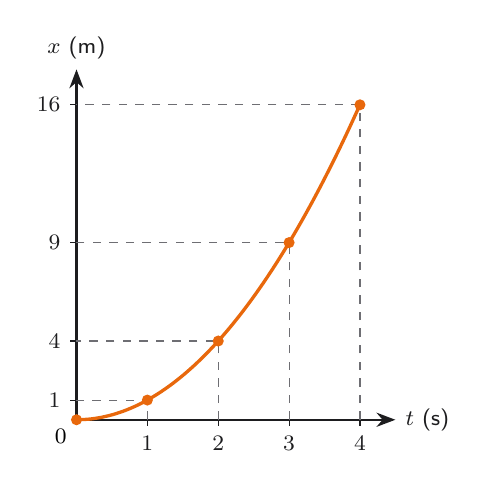
\begin{tikzpicture}[font=\footnotesize,>={Stealth[length=2.4mm]},x=0.9cm,y=0.25cm]
\draw[->,thick,tinta] (0,0) -- (4,0) -- ++(0.45cm,0) node[right] {$t$ (s)};
\draw[->,thick,tinta] (0,0) -- (0,16) -- ++(0,0.45cm) node[above] {$x$ (m)};
\draw[tinta] (1,0) -- ++(0,-0.08cm) node[below] {$1$};
\draw[tinta] (2,0) -- ++(0,-0.08cm) node[below] {$2$};
\draw[tinta] (3,0) -- ++(0,-0.08cm) node[below] {$3$};
\draw[tinta] (4,0) -- ++(0,-0.08cm) node[below] {$4$};
\draw[tinta] (0,1) -- ++(-0.08cm,0) node[left] {$1$};
\draw[tinta] (0,4) -- ++(-0.08cm,0) node[left] {$4$};
\draw[tinta] (0,9) -- ++(-0.08cm,0) node[left] {$9$};
\draw[tinta] (0,16) -- ++(-0.08cm,0) node[left] {$16$};
\node[below left] at (0,0) {$0$};
\draw[very thick,nar,domain=0:4,smooth,variable=\t] plot (\t,{\t*\t});
\draw[dashed,gris] (1,0) -- (1,1) -- (0,1);
\fill[nar] (1,1) circle (2pt);
\draw[dashed,gris] (2,0) -- (2,4) -- (0,4);
\fill[nar] (2,4) circle (2pt);
\draw[dashed,gris] (3,0) -- (3,9) -- (0,9);
\fill[nar] (3,9) circle (2pt);
\draw[dashed,gris] (4,0) -- (4,16) -- (0,16);
\fill[nar] (4,16) circle (2pt);
\fill[nar] (0,0) circle (2pt);
\end{tikzpicture}
\end{document}
